\subsection{Hypothesis on Time Density}
\label{sec:hypothesis_time_density}

\begin{hypothesis}
\label{hyp:time_density}
Prediction quality of queries are higher on queries where the timestamps are in a temporally dense subset of the training dataset, compared to a sparse subset.
\end{hypothesis}

\begin{figure}[htb]
\centering
\begin{minipage}{0.95\columnwidth}
\centering
\small
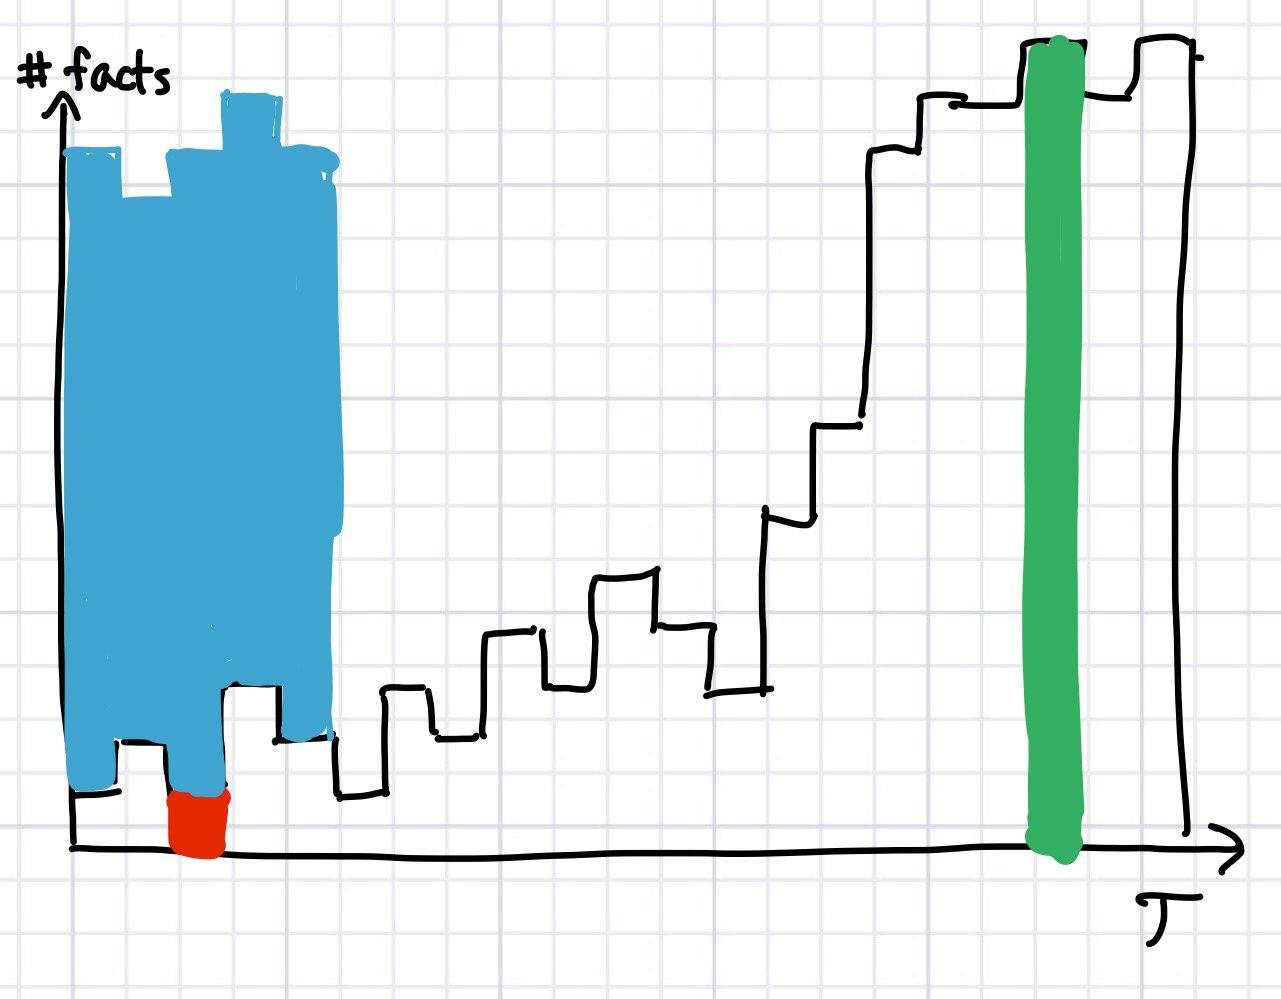
\includegraphics[scale=0.18]{content/hypotheses/figures/time_density.jpg}
\caption{Illustration of \autoref{hyp:time_density}. A dataset with facts sorted by timestamp, timestamp on the Y-axis, fact count on the X-axis.
}
\label{fig:time_density}
\end{minipage}
\end{figure}

This hypothesis is illustrated in \autoref{fig:time_density}. A query from the red bar is expected to have a worse prediction than a query from the green bar because it is in a subset with lower data density. In other words the prediction quality of the same red query would be improved solely by adding facts corresponding to the blue extension of the bars.

It will be examined by creating two partitions of test facts, one where the temporal density is low and one where it is high. The average prediction rank is then found for each partition. If the dense partition has a better overall score, the hypothesis is deemed true.

More specifically, the partitions are created by taking all the facts of a dataset, and depending on the dataset, a temporal granularity is defined based on the granularity and overall density of the dataset. For ICEWS14, the granularity is defined to be days, the same granularity of the dataset itself. For YAGO and Wikidata, the granularity is years. The granularities are defined as timespans $g_1, \dots g_m \in \varT^2$, the first granularity timestamp is less than or equal to any timestamp in the dataset $\timebegin{g_1} \leq \timebegin{\tau}$ where $(h, r, t, \tau) \in \varK$, and the last timestamp is greater than or equal to any beginning timestamp in the dataset $\timeend{g_m} \geq \timebegin{\tau}$ where $(h, r, t, \tau) \in \varK$.

A function $\mathit{num}$ is defined that maps a timestamp to a natural number $\varT \rightarrow \N$. This function describes how many facts that are contained in the granularity timespan that contain that timestamp. The function is defined as

\begin{equation}
\mathit{num}(\tau_x) = \varsum_{(h, r, t, \tau) \in \varK} \I ( \timebegin{g_n} \leq \timebegin{\tau} < \timeend{g_n} )
\end{equation}

where $g_n$ is a granularity timespan, $\timebegin{g_n} \leq \timebegin{\tau_x} < \timeend{g_n}$, and $\I$ is a boolean function that evaluates to $1$ if the containing expression is true, $0$ otherwise.

The median value $d$ is found between all temporal granularity timespans $\mathit{num}(\tau)$ for all timespans $\tau$ in the facts of $\varK$. The dense partition on dataset split $i$ is then defined as

\begin{equation}
P_d = \{ (e_1, r, e_2, \tau) \in \test_i \mid \textit{num}(\tau) \geq \vard \wedge \timebegin{\tau} \neq \varmiss \}
\end{equation}

\noindent
and the sparse partition is defined as 

\begin{equation}
P_s = \{ (e_1, r, e_2, \tau) \in \test_i \mid \textit{num}(\tau) < \vard \wedge \timebegin{\tau} \neq \varmiss \}
\end{equation}

Note that, by these definitions, the facts with missing beginning timestamp is not included, and the partitions are not continuous.

The MRR score of each method is calculated over the $P_d$ and $P_s$ test sets, on several datasets. If the score is significantly higher in $P_d$, the hypothesis is true, and if the score is signigicantly higher in $P_s$ the hypothesis is false.
